\documentclass{article}
\usepackage[T1]{fontenc}
\usepackage[utf8]{inputenc}
\usepackage[french]{babel}
\usepackage{enumitem}
\usepackage{amsmath}
\usepackage{amssymb}
\usepackage{graphicx}
\usepackage{listings}
\usepackage{hyperref}
\usepackage[dvipsnames]{xcolor}
\setcounter{tocdepth}{2}
\hypersetup{
    colorlinks,
    citecolor=black,
    filecolor=black, 
    linkcolor=black,
    urlcolor=black
}

\lstset{language=Python,
        basicstyle=\ttfamily,
        keywordstyle=\color{BlueViolet}\ttfamily,
        commentstyle=\color{OliveGreen}\ttfamily,
        breaklines=true,
}

\title{Rapport du devoir maison de Sécurité}
\author{BASUALDO Lautaro et LOI Léo}

\begin{document}
\maketitle

\tableofcontents
\newpage

\section{Exercice 1 :}

    Avant de pouvoir décrypter les deux mots de passes, nous devons déjà les identifier.\\
    Or, nous savons que la fonction SHA-256 génèrera toujours le même haché pour un mot de passe donné.\\
    Ainsi, nous pouvons détecter deux hachés différents :
    \begin{itemize}
        \item 068be8be83f9bfafd1545d357fd3cd132f8c659effd11e635a698811b796c880\\
        (utilisé par Bart, Homer, Lisa et March)
        \item 15e2b0d3c33891ebb0f1ef609ec419420c20e320ce94c65fbc8c3312448eb225\\
        (utilisé par Bob, Carlton, John et William)
    \end{itemize}

    Pour le premier haché, grâce aux différents indices, nous pouvons deviner que le mot de passe utilisé est le 74ème élément du tableau périodique des élements. A savoir le "tungstène" appelé en anglais "tungsten"\\
    Afin de s'assurer de nos résultats, nous avons haché le mot "tungsten" avec la fonction de hachage SHA-256 ce qui donne le résultat suivant :\\
    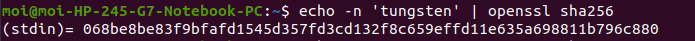
\includegraphics[scale = 0.5]{tungsten.png}
    Nous pouvons constater que les deux hachés sont similaire, le mot de passe utilisé par Bart, Homer, Lisa et March est donc bien "tungsten"\medskip

    Pour le second haché, grâce aux différents indices, nous pouvons deviner que le mot de passe utilisé est la suite de chiffres "123456789"\\
    Afin de s'assurer de nos résultats, nous avons haché le mot "123456789" avec la fonction de hachage SHA-256 ce qui donne le résultat suivant :\\
    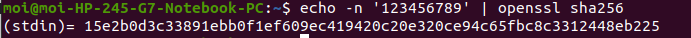
\includegraphics[scale = 0.5]{chiffre.png}
    Nous pouvons constater que les deux hachés sont similaire, le mot de passe utilisé par Bob, Carlton, John et William est donc bien "123456789"
\newpage
\section{Exercice 2 :}
    \subsection{Question 1 :}
        \lstinputlisting[linerange={8-46}]{ui.py}
    \subsection{Question 2 :}
        Après plusieurs éxecutions du programme ci-dessus, les valeurs suivantes peuvent être récupérées dans la base de donnée\newline
        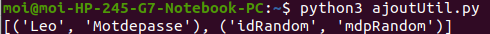
\includegraphics[scale = 0.5]{ajoutUtil.png}
    \subsection{Question 3 :}
        \lstinputlisting[linerange={54-67}]{ui.py}
    \subsection{Question 4 :}
        Notre fonction d'AjoutUtilisateur renvoyant une liste contenant l'identifiant et le mot de passe de l'utilisateur,
        il nous suffit de récupérer ces données, et de les renvoyer une fois le mot de passe haché
        \lstinputlisting[linerange={74-79}]{ui.py}
    \subsection{Question 5 :}
        \lstinputlisting[linerange={82-87}]{ui.py}
    \subsection{Question 6 :}
        \lstinputlisting[linerange={89-98}]{ui.py}
\newpage
\section{Exercice 3 :}
    \subsection{Question 1 :}
        Grâce aux logs que nous avons pû récupérer, nous pouvons réussir à identifier plusieurs informations concernant l'attaque.\newline
        On peut tout d'abord repérer que l'attaque bruteforce a commencé à 8h58 et 35 secondes.
        On peut l'identifier car à partie de la ligne 268 des logs, nous pouvons observer un nombre anormal de requêtes qui sont toutes efféctuées dans un laps de temps très court.
    \subsection{Question 2 :}
        Nous pouvons voir à partir de la ligne 1321 jusqu'à la ligne ... que l'attaquant répète les 2 même requêtes en changeant uniquement l'extension.
        Il utilise les extensions :
        \begin{itemize}
            \item .php
            \item .phmtl
            \item .php3
            \item .php4
            \item .php5
            \item .php6
            \item .php7
            \item .phar
        \end{itemize}
    \subsection{Question 3 :}
        Il s'arrête à l'extension .phar, ayant sûrement trouvé une faille pour s'introduire dans le système grâce à cette extension.
        Il s'agit aussi de l'extension qu'il utilisera pour le reste de ses requêtes.
    \subsection{Question 4 :}
        Nous pouvons voir que l'attanquant utilise le fichier php pour exécuter les commandes suivantes :
        \begin{description}
            \item[Ligne 1340 :] Il télécharge un fichier fiche\_de\_poste.odt.
            \item[Ligne 1341 :] 
            \item[Ligne 1342 :] Il modifie les droits d'accès au ficheir qu'il vient de déplacer.
            \item[Ligne 1343 :] Il entre dans le fichier afin, possiblement, d'en récupérer les données.
        \end{description}
\section{Exercice 4 :}
    \subsection{Question 1 :}
        Après un peu de recherche, nous avons trouvé que les SMS/MMS sont stockés dans une base de donnée nommée : \textbf{mms.sms.db}\newline
        Son chemin est le suivant : $filesystem/data/user\_de/0/com.android.providers.telephony/databases$
    \subsection{Question 2 :}
        Nous avons trouvé deux messages parlant d'identifiants. Voici les informations les concernant : 
        \begin{itemize}
            \item ID : 148\newline
             date : 1683893316000 = vendredi 12 mai 2023 12:08:36\newline
             contenu : Bonjour à tous, petit message collectif pour vous annoncer que les identifiants de tous les utilisateurs de l’intranet vont être changé d’ici 2 semaines. Je reviendrais vers vous lorsque le changement aura lieu. Bonne journée.
            \item ID : 151\newline
             date : 1684736105000 = lundi 22 mai 2023 06:15:05\newline
             contenu : Bonjour tout le monde, le changement des identifiants viens d’avoir lieu, vous trouverez dans l’image jointe vos nouveaux identifiants. N’hésitez pas si vous rencontrez des problèmes. Bonne journée.
        \end{itemize}
    \subsection{Question 3 :}
        Nous savons désormais que les identifiants ont été envoyés dans une image jointe à un message. 
        Un tout petit peu de recherche nous permet de retrouver l'image ci-dessous à l'adresse :\newline
        $filesystem/data/user\_de/0/com.android.providers.telephony/app\_parts$\newline
        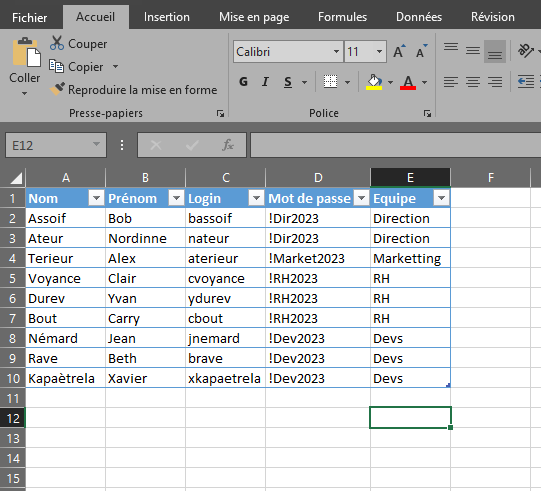
\includegraphics[scale=0.5]{id.jpg}\newline
        Il est donc très facile désormais de trouver que le mot de passe associé aux RH est "!RH2023"
    \subsection{Question 4 :}
        
    \subsection{Question 5 :}
        En cherchant, nous pouvons trouver un fichier contenant la base de données du calendar.
        En regardant les events à l'intérieur, nous trouvons un évènement nommé "Réparation téléphonique" le  
\end{document}